\documentclass{scrartcl}

% Adapted from an original template by Hlyni Arnórssyni, Reykjavik University, Iceland
%
% ------------------------------ SETTINGS
\usepackage{geometry}

\geometry{
    paper=a4paper, % Paper size
    top=2.5cm, % Top margin
    bottom=2.5cm, % Bottom margin
    left=2.5cm, % Left margin
    right=2.4cm, % Right margin
    headheight=0.75cm, % Header height
    footskip=1.5cm, % Space from the bottom margin to the baseline of the footer
    headsep=0.75cm, % Space from the top margin to the baseline of the header
    %showframe, % Uncomment to show how the type block is set on the page
}

\usepackage{blindtext}
%-------------------------------- Character encoding ----------------------------
\usepackage[T1]{fontenc}
\usepackage[utf8]{inputenc}

%----------------------------- Mathematics packages from AMS ---------------

\usepackage{amsmath, amsfonts, amsthm, amssymb}
\usepackage{braket, nicefrac}

% ----------- International System of Units
\usepackage{siunitx}

%------------------------------ Lists / numbers -------------------------
\usepackage{enumitem, multicol}

%------------------------------- Figure insertions --------------
\usepackage{graphicx, float}  % Use option [H] to force the placement of a figure
\usepackage{keystroke}
\usepackage{pgfplots}\usepgfplotslibrary{units}\pgfplotsset{compat=1.16}

%------------------------------- Line Spacing --------------
\usepackage{setspace}

%------------------------------- Depth of the ToC --------------
\setcounter{tocdepth}{2}

%%%%%%%%%%%%%%%%%%%%%%%%%% Hyperlink References %%%%%%%%%%%%%%%%%%%%%%%%%%%
\usepackage{hyperref}

\usepackage{listings}
\usepackage{textcomp}
\lstset{upquote=true}

%--------------------% Storage Path for images %-----------------%
\graphicspath{{graphics/}{Graphics/}{./}}

%%%%%%%%%%%%%%%%%%%%%%%%%% Environments %%%%%%%%%%%%%%%%%%%%%%%%%%%
\renewenvironment{abstract}{
    \begin{center}
        \textbf{Abstract}
        \vspace{0.5cm}
        \par\itshape
        \begin{minipage}{0.8\linewidth}}{\end{minipage}
        \noindent\ignorespaces
    \end{center}
}

\newenvironment{keywords}{
    \begin{center}
        \textbf{Keywords}
        \vspace{0.5cm}
        \par
        \begin{minipage}{0.8\linewidth}}{\end{minipage}
        \noindent\ignorespaces
    \end{center}
}

\newenvironment{preface}{
    \begin{center}
        \textbf{Preface}
        \vspace{0.5cm}
        \par
        \begin{minipage}{0.8\linewidth}}{\end{minipage}
        \noindent\ignorespaces
    \end{center}
}

\newenvironment{acknowledgements}{
    \begin{center}
        \textbf{Acknowledgements}
        \vspace{0.5cm}
        \par
        \begin{minipage}{0.8\linewidth}}{\end{minipage}
        \noindent\ignorespaces
    \end{center}
}

\usepackage{spalign}

\newcommand{\code}[1]{\texttt{#1}}

\begin{document}
%Title of the report, name of coworkers and dates (of experiment and of report).
\begin{titlepage}
    \centering
    {\large \today\par}
    \vfill

    %%%% PROJECT TITLE
    {\huge\bfseries Differential Swerve State Space Controller Design\par}
    \vfill

    %%%% AUTHOR(S)
    {\Large\itshape Henry LeCompte}\par
    {\itshape FRC Team 2383, The Ninjineers}\par
    \vspace{1.5cm}

    \vfill
    % Bottom of the page
\end{titlepage}

\newpage

\doublespacing
\tableofcontents
\singlespacing

\newpage

\doublespacing

\section{Introduction}
\subsection*{What is Swerve?}
Swerve is a type of drivetrain that is characterized by having at least two wheels that can each rotate and spin independently of each other (here rotate is define as a rotation around the robots up axis and spin is defined as a rotation around the modules y axis). This allows the robot to move in any direction and turn in place. Differential Swerve is a type of swerve drivetrain in which the rotation of the wheel is controlled by the difference of the motor velocities and the spin if the wheel is controlled by the average of the motor velocities. This allows for the combination of the torque produced by both motors when driving and turning. This is the main advantage over conventional (coaxial) swerve drivetrains in which rotation and spin are controlled by separate motors. The main disadvantage of differential swerve is that it is significantly more complex to control.

\subsection{Purpose of this paper}
By reading this paper you should be able to gain an understanding of how a relatively complex mechanism is analyzed and a state space model is created. You should then learn the steps to implement a simple Linear Quadratic Regulator (LQR) and then a Kalman Filter to filter out measurement noise.

\subsection{Who should read this paper}
This paper was designed for High School students currently competing in First Robotics Competition (FRC) although nothing in this paper is specific to this competition, swerve is commonly used in this competition and it provides many tools for state-space controls.

\newpage
\section{Designing the State Space Model}

We need to design a continuous, time-invariant state space model of the system. This will allow us to estimate the response of the system to create a feedforward and feedback controller. The following is the general form of a state space model.
\begin{equation} \label{state-change}
    \dot{x} = Ax + Bu
\end{equation}
\begin{equation} \label{output}
    y = Cx + Du
\end{equation}

\subsection*{What should we choose as our inputs, outputs, and states?}
\subsubsection*{Inputs}
In robotics you can commonly only input one value, voltage, but because differential swerve has two motors that work together to control the module we can pass in two inputs, the top motor input and the bottom motor input. In differential swerve we refer to the motors as top and bottom because there is one motor that drives the top gear of the differential and there is one motor that drives the bottom gear of the differential not because one of the motors is physically on top of the other.

\subsubsection*{Outputs}
Outputs in a state-space model are things that you can physically measure. Although, this makes it a little confusing as to what we should chose because there are many different things we can measure with each encoder (displacement, velocity, acceleration) and we have 3 of them. To figure out what to output we need to think about which of these is it actually important for us to measure.
In swerve there are really two things that we need to know: the velocity of the wheel, and the rotation of the wheel. Even though it would be nice to have these as outputs we only have a way of directly measuring one of these with the module rotation encoder. For the wheel velocity we can instead output the velocity of both motors, we can then calculate the wheel velocity as the average of the motor speeds.
So we are going to have three outputs: top motor velocity[radians/second], bottom motor velocity [radians/second], and wheel rotation [radians]

\subsubsection*{States}
To calculate the change in the state of the system we can only use the states and the inputs. We might be able to see that we can calculate how the output variables will change just by knowing the the current outputs and the inputs, this means that we can use these as the states. We now have the same states as outputs which means that our C matrix will be the identity matrix and our D matrix will be 0.

\subsection{Inputs, Outputs, and States}
The States will be in the form of
\begin{equation}
    x =
    \begin{bmatrix}
        v_t    \\
        v_b    \\
        \theta \\
    \end{bmatrix}
\end{equation}

Where \(\theta\) is the angle of the wheel and\(v_t\) and \(v_b\) are the top and bottom motor velocities respectively. \\
The velocity of the wheel is not included as a state because it is a linear combination of the motor velocities so it can be calculated from the current state.

The inputs will be in the form of
\begin{equation}
    u =
    \begin{bmatrix}
        V_t \\
        V_b \\
    \end{bmatrix}
\end{equation}

Where \(V_t\) is the top motor voltage and \(V_b\) is the bottom motor voltage.

Our output matrix is the same as the state matrix as we can measure all states.
\begin{equation}
    y =
    \begin{bmatrix}
        v_t \\
        v_b \\
        \theta
    \end{bmatrix}
\end{equation}

Where \(v_t\) is the top motor velocity, \(v_b\) is the bottom motor velocity, and \(\theta\) is the angle of the wheel.

\subsection{DC Motor Model}
We know that a permanent magnet DC motor follows the general equation of
\begin{equation}
    V = K_v\dot{x} + K_a\ddot{x}
\end{equation}
And we can rewrite this as
\begin{align*}
    V               & = K_v\dot{x} + K_a\ddot{x}                \\
    V - K_a\ddot{x} & = K_v\dot{x}                              \\
    -K_a\ddot{x}    & = K_v\dot{x} - V                          \\
    \ddot{x}        & = \frac{-K_v\dot{x} + V}{K_a}             \\
    \ddot{x}        & = \frac{-K_v\dot{x}}{K_a} + \frac{V}{K_a}
\end{align*}
We can also substitute v as \(\dot{x}\) to create
\begin{equation}
    \dot{v} = \frac{-K_v v}{K_a} + \frac{V}{K_a}
\end{equation}

This equation can then be written in state space form as
\begin{equation}
    \dot{x} = \begin{bmatrix}\frac{-K_v}{K_a}\end{bmatrix}x + \begin{bmatrix}\frac{1}{K_a}\end{bmatrix}u
\end{equation}
\begin{equation}
    y = 1x + 0u
\end{equation}

\subsection{A and B Matrices}
Now that we know how to calculate the angular velocity of a motor based on its constants and the input voltage we can start to create the formulas needed to compute the different velocity components of the system.
\begin{align}
    \dot{v_t}    & = \frac{-K_{v_\mathit{drive}}}{K_{a_\mathit{drive}}}v_t + \frac{1}{K_{a_\mathit{drive}}}V_t \\
    \dot{v_b}    & = \frac{-K_{v_\mathit{drive}}}{K_{a_\mathit{drive}}}v_b + \frac{1}{K_{a_\mathit{drive}}}V_b \\
    \dot{\theta} & = \frac{v_t + v_b}{2} * K_\mathit{turn\_ratio}
\end{align}

We can now rewrite these equations as a system that has coefficients for every state and input.
\begin{align}
    \dot{v_t}    & = \frac{-K_{v_\mathit{drive}}}{K_{a_\mathit{drive}}}v_t + 0v_b + 0\theta + \frac{1}{K_{a_\mathit{drive}}}V_t + 0V_b                                                                                  \\
    \dot{v_b}    & = 0v_t + \frac{-K_{v_\mathit{drive}}}{K_{a_\mathit{drive}}}v_b + 0\theta + 0V_t + \frac{1}{K_{a_\mathit{drive}}}V_b                                                                                  \\
    \dot{v_w}    & = -\frac{K_{v_\mathit{drive}}}{2K_{a_\mathit{drive}}}v_t + \frac{K_{v_\mathit{drive}}}{2K_{a_\mathit{drive}}}v_b + 0\theta + \frac{1}{2K_{a_\mathit{drive}}}V_t - \frac{1}{2K_{a_\mathit{drive}}}V_b \\
    \dot{\theta} & = \frac{K_\mathit{turn\_ratio}}{2}v_t + \frac{K_\mathit{turn\_ratio}}{2}v_b + 0\theta + 0V_t + 0V_b
\end{align}

Now that we have these linear equations we can turn them into the A and B matrix.

\begin{align}
    A & =
    \begin{bmatrix}
        \frac{-K_{v_\mathit{drive}}}{K_{a_\mathit{drive}}} & 0                                                  & 0 \\
        0                                                  & \frac{-K_{v_\mathit{drive}}}{K_{a_\mathit{drive}}} & 0 \\
        \frac{K_\mathit{turn\_ratio}}{2}                   & \frac{K_\mathit{turn\_ratio}}{2}                   & 0 \\
    \end{bmatrix} \\
    B & =
    \begin{bmatrix}
        \frac{1}{K_{a_\mathit{drive}}} & 0                              \\
        0                              & \frac{1}{K_{a_\mathit{drive}}} \\
        0                              & 0                              \\
    \end{bmatrix}
\end{align}

\subsection{C and D matrices}
With these, we just need the C and D matrices.
Because the output matrix is the same as the state matrix C is just the identity matrix.
\begin{align}
    C & =
    \begin{bmatrix}
        1 & 0 & 0 \\
        0 & 1 & 0 \\
        0 & 0 & 1 \\
    \end{bmatrix} \\
    D & = 0
\end{align}

\subsection{Full model}
And now will all of these matrices we can write the full continuous model as
\begin{equation}
    \dot{\begin{bmatrix}
            v_t    \\
            v_b    \\
            \theta \\
        \end{bmatrix}} =
    \begin{bmatrix}
        \frac{-K_{v_\mathit{drive}}}{K_{a_\mathit{drive}}} & 0                                                  & 0 \\
        0                                                  & \frac{-K_{v_\mathit{drive}}}{K_{a_\mathit{drive}}} & 0 \\
        \frac{K_\mathit{turn\_ratio}}{2}                   & \frac{K_\mathit{turn\_ratio}}{2}                   & 0 \\
    \end{bmatrix}\begin{bmatrix}
        v_t    \\
        v_b    \\
        \theta \\
    \end{bmatrix} + \begin{bmatrix}
        \frac{1}{K_{a_\mathit{drive}}} & 0                              \\
        0                              & \frac{1}{K_{a_\mathit{drive}}} \\
        0                              & 0                              \\
    \end{bmatrix}\begin{bmatrix}
        V_t \\
        V_b \\
    \end{bmatrix}
\end{equation}
\begin{equation}
    \begin{bmatrix}
        v_t    \\
        v_b    \\
        \theta \\
    \end{bmatrix}      = \begin{bmatrix}
        1 & 0 & 0 \\
        0 & 1 & 0 \\
        0 & 0 & 1 \\
    \end{bmatrix}\begin{bmatrix}
        v_t    \\
        v_b    \\
        \theta \\
    \end{bmatrix} + 0\begin{bmatrix}
        V_t \\
        V_b \\
    \end{bmatrix}
\end{equation}

Now we can also add the following constants to the model (These will be different for each robot)
\begin{align}
    K_{v_\mathit{drive}}   & = 0.023        \\
    K_{a_\mathit{drive}}   & = 0.001        \\
    K_\mathit{turn\_ratio} & = \frac{1}{28}
\end{align}

\newpage

\section{Validating the State Space Model}
Now that we have a state space model we need to validate that it is controllable, observable and stable.
\subsection{Controllability}
Controllability is a property of the system that allows any initial state to be driven to any desired state using control inputs in a finite time.
The Controllability matrix for continuous time-invariant systems is defined as
\begin{equation}
    \mathit{R} = \begin{bmatrix}
        B & AB & A^2B & \dots & A^{n-1}B
    \end{bmatrix}
\end{equation}
And the system is said to be controllable if the rank of the controllability matrix is equal to the number of states (n).
\begin{equation}
    \mathit{rank}(\mathit{R}) = n
\end{equation}

We can now calculate the rank of the controllability matrix for our system and find that it is indeed 3. This means that out system is indeed controllable and we can move on to the next step.

\subsection{Observability}
A system is said to be observable if, for every possible state, the current state can be estimated using only the information from outputs.
The observability matrix for continuous time-invariant systems is defined as
\begin{equation}
    \mathit{O} = \begin{bmatrix}
        C      \\
        CA     \\
        CA^2   \\
        \vdots \\
        CA^{n-1}
    \end{bmatrix}
\end{equation}

And the system is said to be observable if the rank of the observability matrix is equal to the number of states (n).

\begin{equation}
    \mathit{rank}(\mathit{O}) = n
\end{equation}

Calculating this for our current system we find that the rank is 3. This means that our system is observable and we can move on to the next step.

\subsection{Stability}
A system is said to be stable if the eigenvalues of the A matrix are all negative.
Calculating the eigenvalues of the A matrix we can find that the real parts of the eigenvalues are 0 and -23. This means that our system is marginally stable but we can fix this with the LQR controller in the next section.

\subsection{Step Response}
To validate that our system is stable we can also look at the step response of the system.
The step response is the response of the system to a step input.
This can be calculated with the python package control.
We can graph the step response values for the system and find that the system is indeed stable. This graph can be seen in figure \ref{fig:step_response}.

\subsection{Forced Response}
We also want to make sure that the wheel is turning correctly and is still stable with different inputs. To do this we can create a graph of forced inputs. This graph uses 5 time steps of 12 volts on each motor. 495 more time steps of 12 and -12 volts and 500 more time steps of no voltage. This graph can be seen in figure \ref{fig:forced_response}.

\begin{minipage}{.45\textwidth}
    \centering
    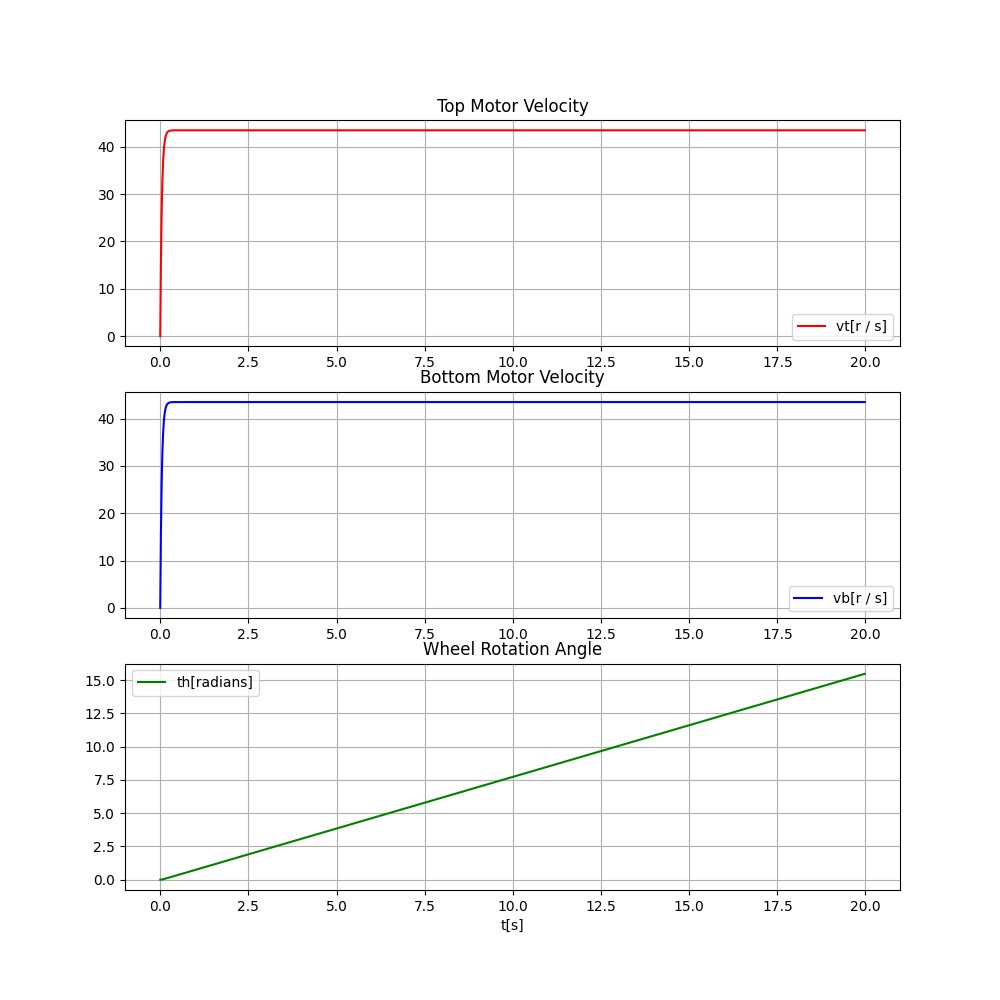
\includegraphics[width=\textwidth]{step_response.png}
    \captionof{figure}{Step response of the system}
    \label{fig:step_response}
\end{minipage}
\begin{minipage}{.45\textwidth}
    \centering
    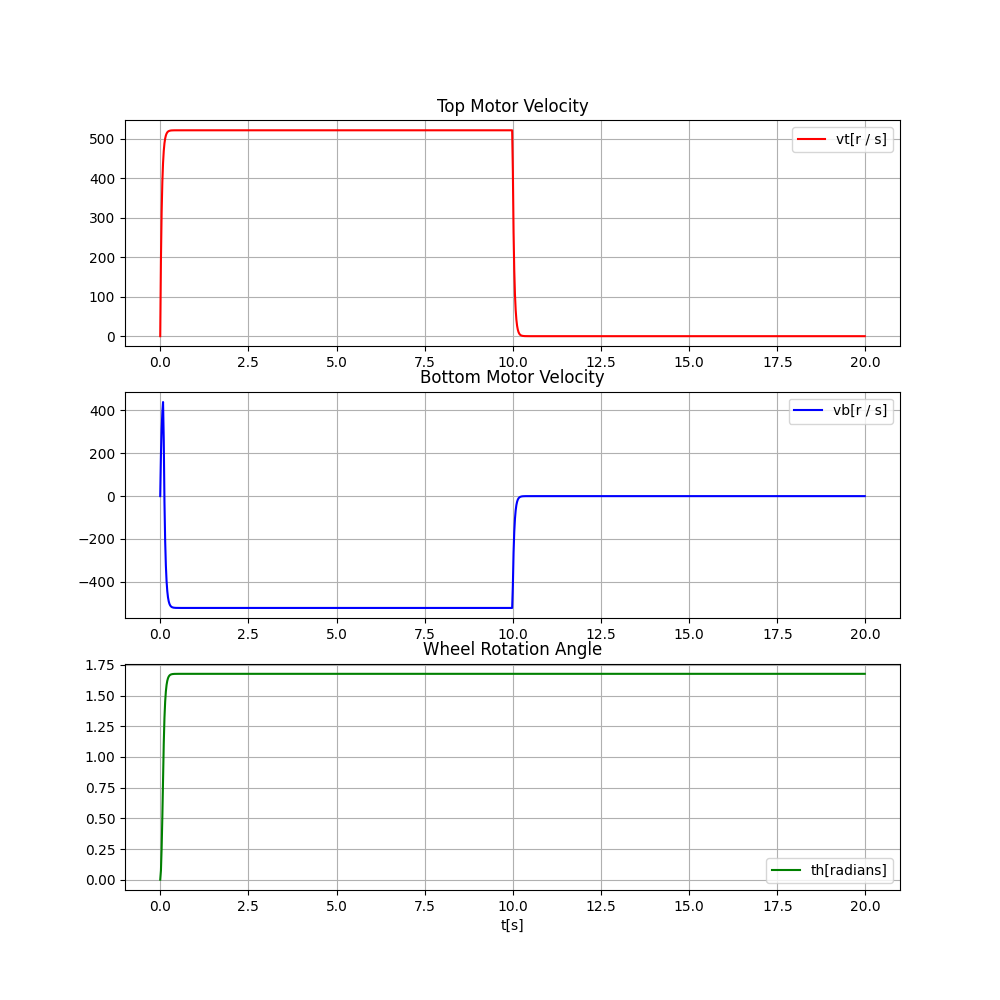
\includegraphics[width=\textwidth]{forced_response.png}
    \captionof{figure}{Forced response of the system}
    \label{fig:forced_response}
\end{minipage}

\newpage

\end{document}
